% SPDX-FileCopyrightText: 2026 Cyprien PIERRE
% SPDX-License-Identifier: CC-BY-4.0
\documentclass[tikz,border=5pt]{standalone}
\usepackage[T1]{fontenc}
\usepackage{lmodern}
\usetikzlibrary{arrows.meta,positioning}
\begin{document}
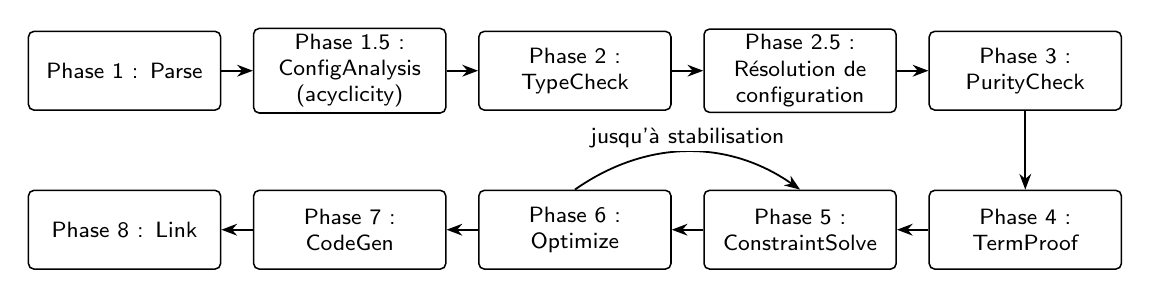
\begin{tikzpicture}[
  font=\sffamily\footnotesize,
  phase/.style={draw, rounded corners=2pt, align=center, minimum height=10mm,
    text width=23mm, inner sep=2pt, line width=.55pt},
  flow/.style={-{Stealth[length=2mm]}, line width=.65pt},
  node distance=4mm
]
\node[phase] (parse) {Phase 1 : Parse};
\node[phase, right=of parse] (config) {Phase 1.5 : ConfigAnalysis\\(acyclicity)};
\node[phase, right=of config] (type) {Phase 2 : TypeCheck};
\node[phase, right=of type] (resolve) {Phase 2.5 : Résolution de configuration};
\node[phase, right=of resolve] (purity) {Phase 3 : PurityCheck};
\node[phase, below=10mm of purity] (proof) {Phase 4 : TermProof};
\node[phase, left=of proof] (constraints) {Phase 5 : ConstraintSolve};
\node[phase, left=of constraints] (optimize) {Phase 6 : Optimize};
\node[phase, left=of optimize] (codegen) {Phase 7 : CodeGen};
\node[phase, left=of codegen] (link) {Phase 8 : Link};
\draw[flow] (parse) -- (config);
\draw[flow] (config) -- (type);
\draw[flow] (type) -- (resolve);
\draw[flow] (resolve) -- (purity);
\draw[flow] (purity.south) -- (proof.north);
\draw[flow] (proof.west) -- (constraints.east);
\draw[flow] (constraints.west) -- (optimize.east);
\draw[flow] (optimize.north) to[bend left=35] node[above, fill=white, inner sep=1pt] {jusqu'à stabilisation} (constraints.north);
\draw[flow] (optimize.west) -- (codegen.east);
\draw[flow] (codegen.west) -- (link.east);
\end{tikzpicture}
\end{document}